% !TeX root = ../main.tex
\section{Результаты расчетов и моделирования}

\subsection{Зависимости СКО фильтрации и полосы ЧАП в установившемся режиме}
На рис.~\ref{fig:analytic_q} приведены зависимости установившегося СКО ошибки фильтрации частоты $\sigma_\Omega$ и оптимальной эквивалентной шумовой полосы $\Delta F_{\text{ЧАП}}$ от отношения сигнал/шум $q_{c/n_0} \in [14, 50]\text{ дБГц}$ при фиксированном ускорении $\sigma_a = 10\text{ м/с}^2$. На рис.~\ref{fig:analytic_a} показаны аналогичные зависимости от среднеквадратического ускорения $\sigma_a \in [1, 30]\text{ м/с}^2$ при $q_{c/n_0} = 30\text{ дБГц}$.

\begin{figure}[H]
\centering
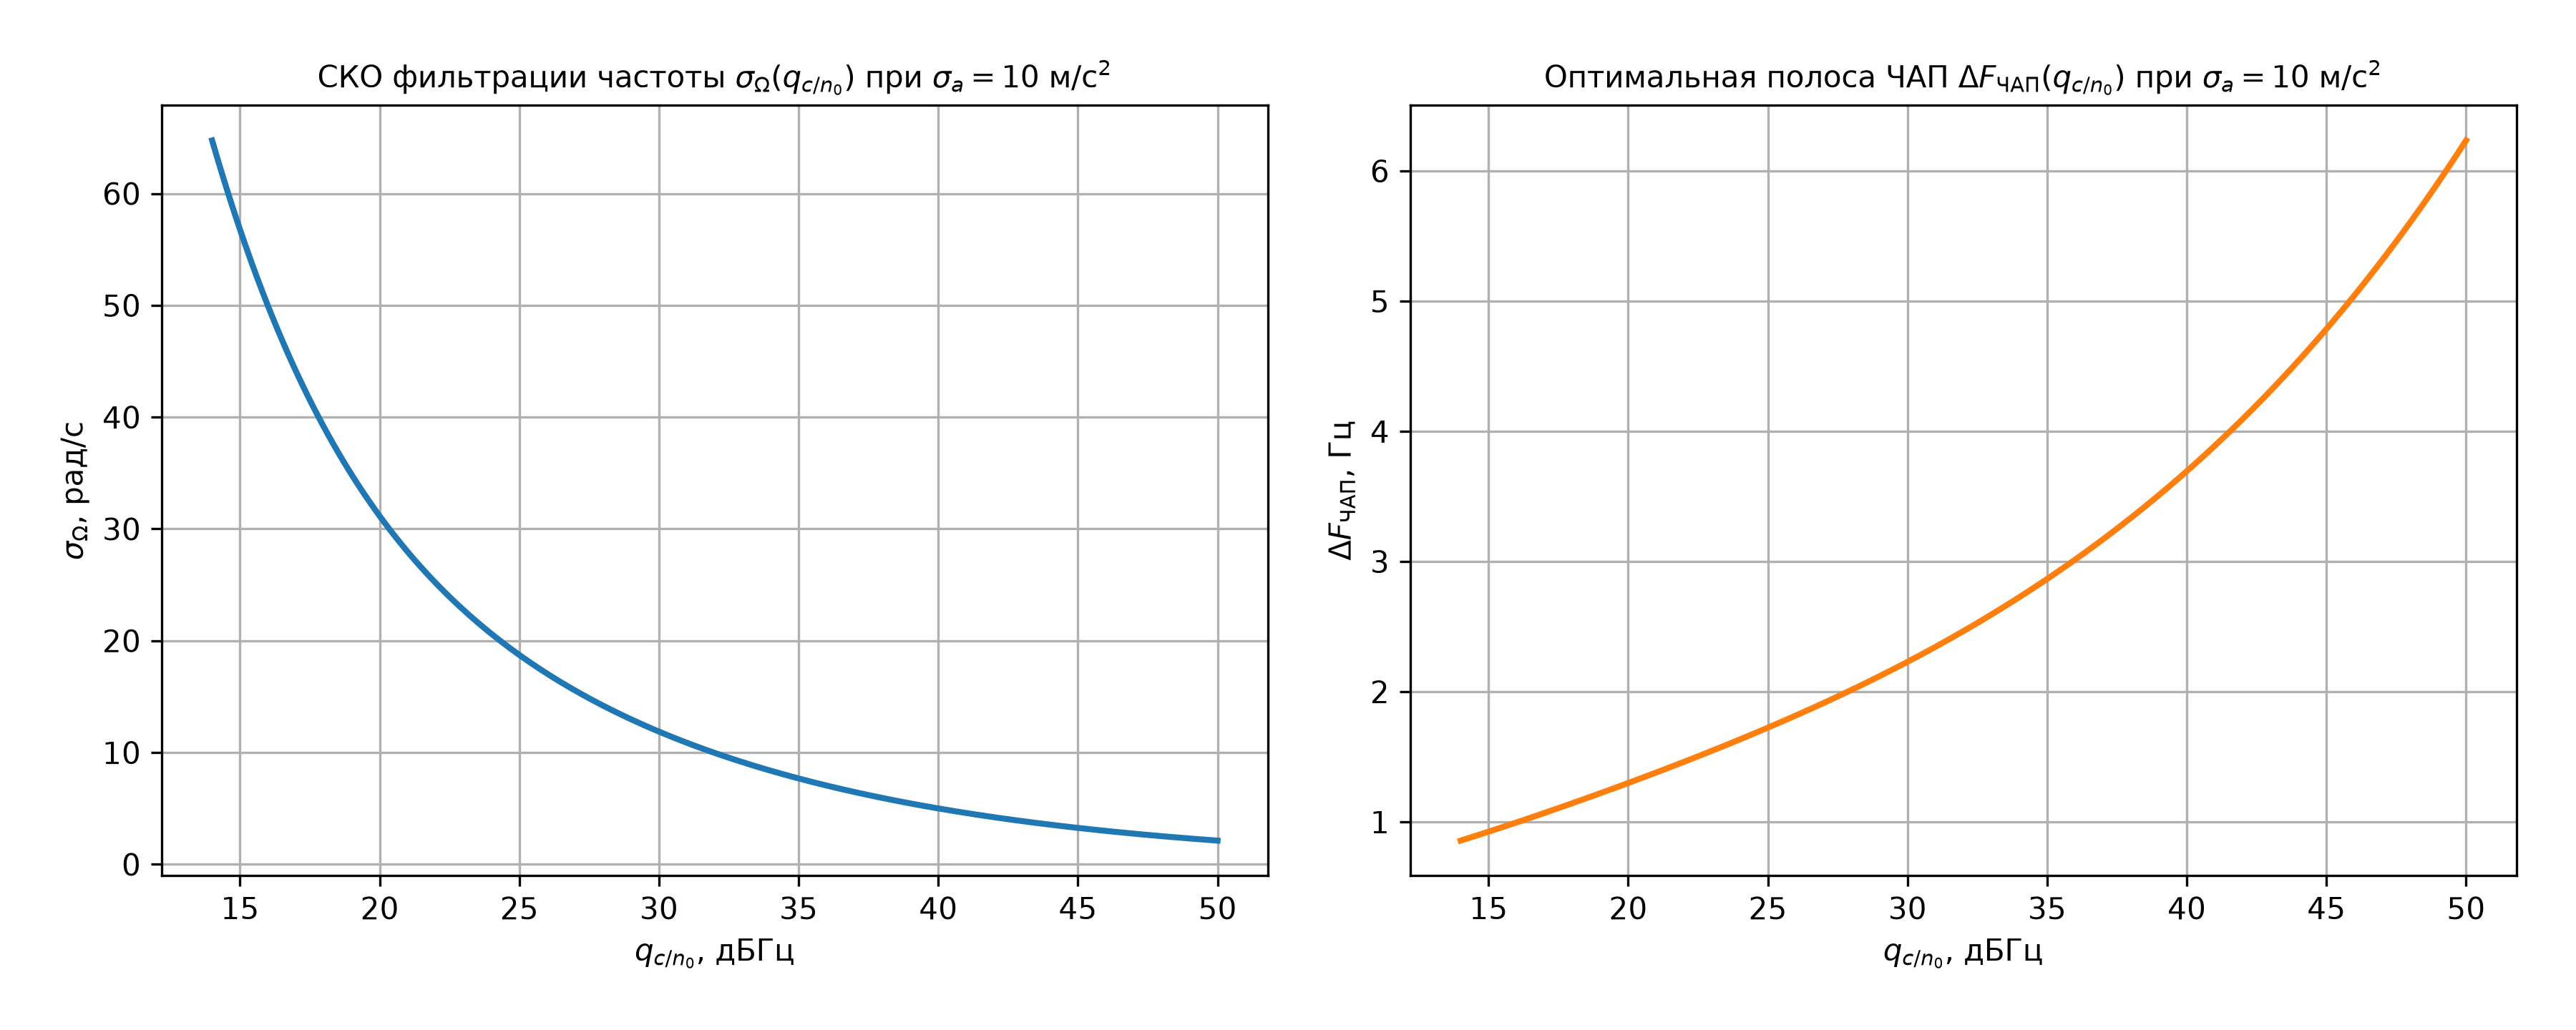
\includegraphics[width=0.95\textwidth]{4.png}
\caption{Зависимости СКО фильтрации $\sigma_\Omega$ и полосы $\Delta F_{\text{ЧАП}}$ от отношения $q_{c/n_0}$ при $\sigma_a = 10\text{ м/с}^2$}
\label{fig:analytic_q}
\end{figure}

\begin{figure}[H]
\centering
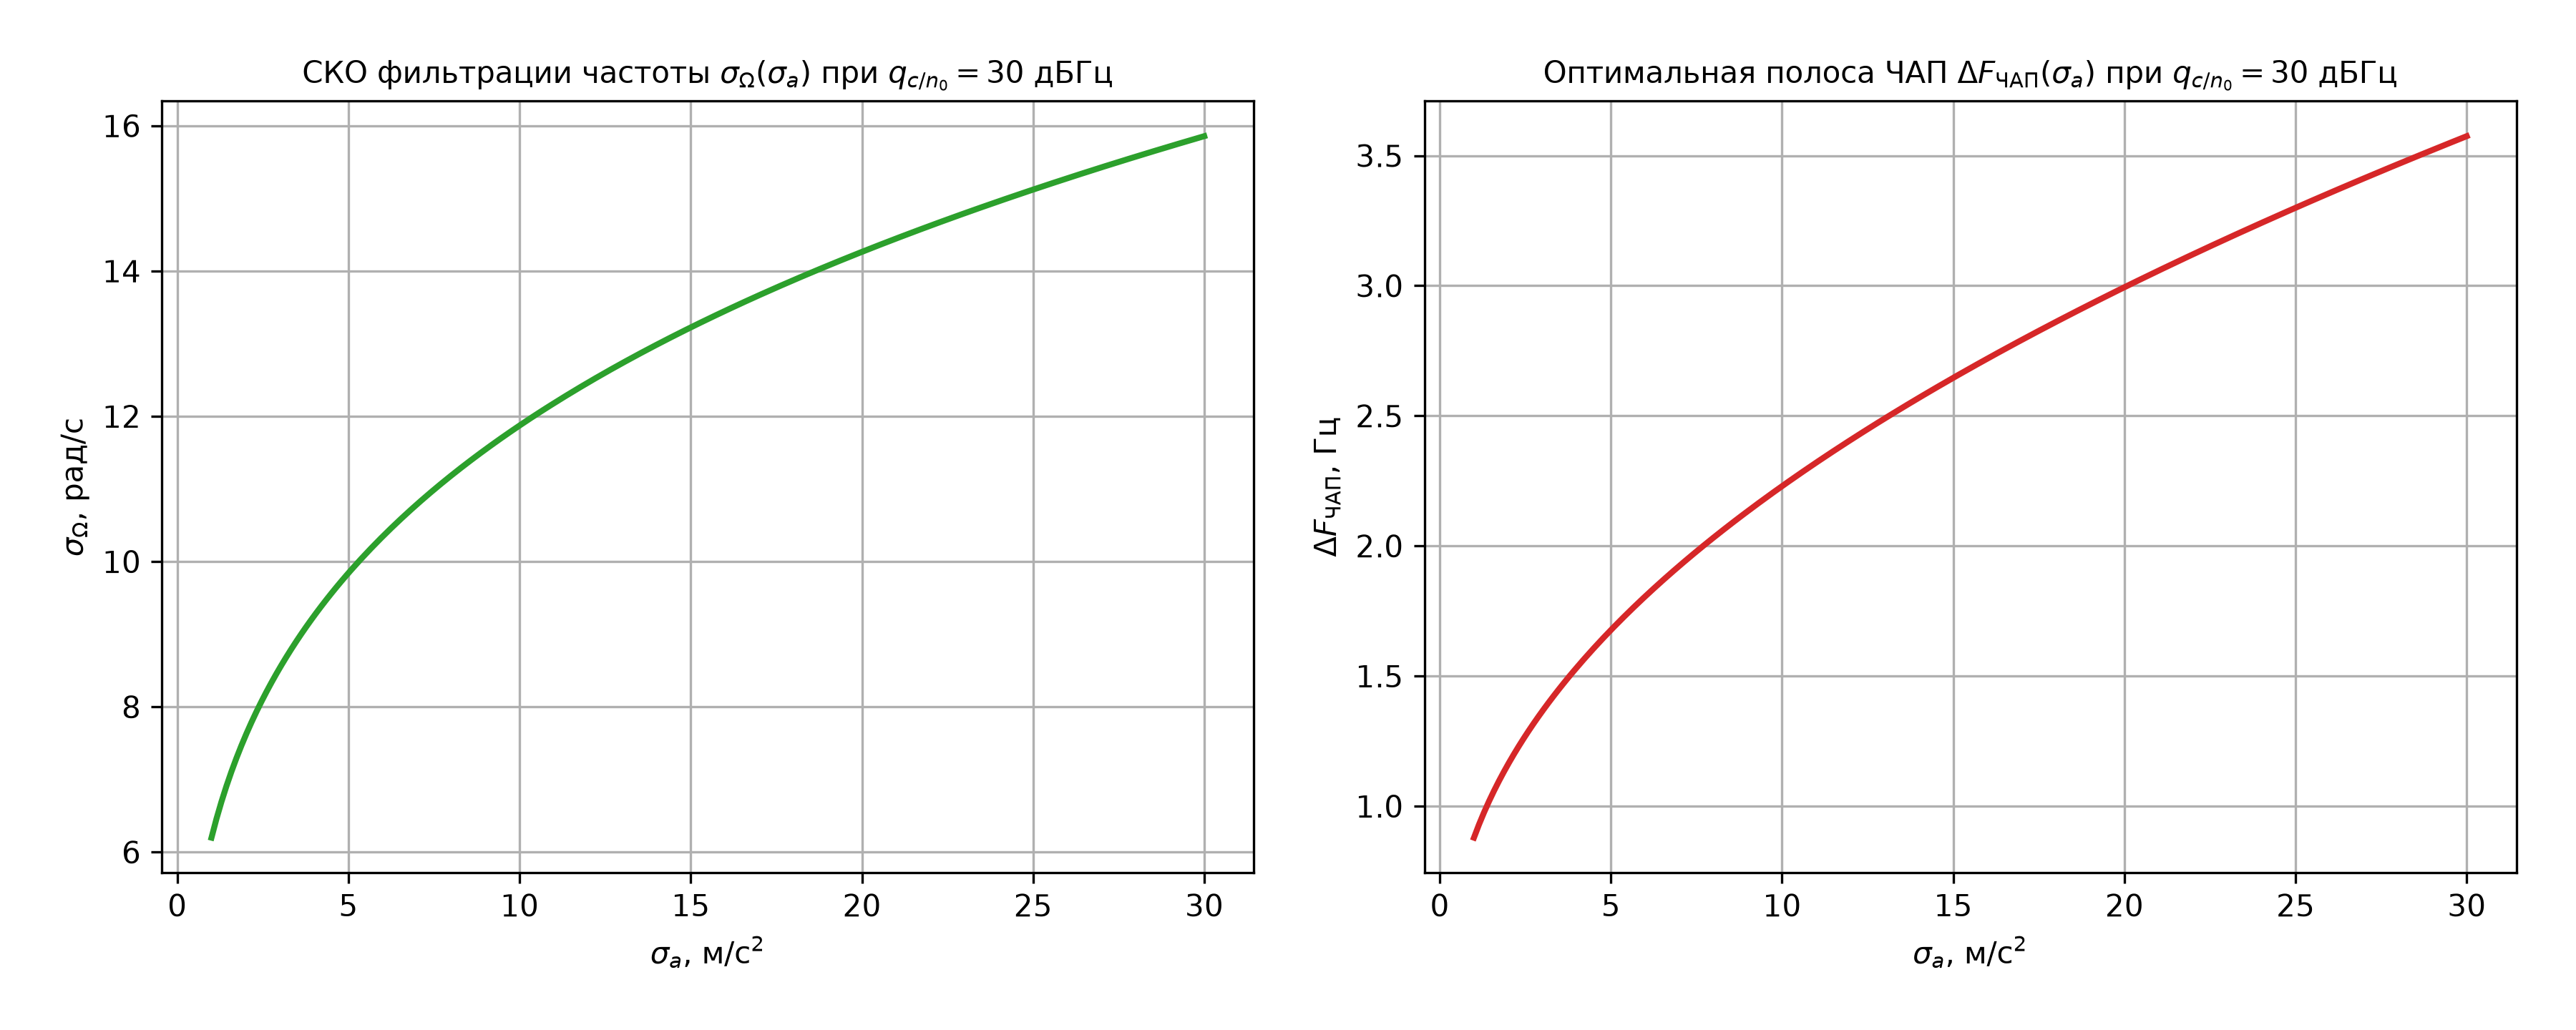
\includegraphics[width=0.95\textwidth]{5.png}
\caption{Зависимости СКО фильтрации $\sigma_\Omega$ и полосы $\Delta F_{\text{ЧАП}}$ от ускорения $\sigma_a$ при $q_{c/n_0} = 30\text{ дБГц}$}
\label{fig:analytic_a}
\end{figure}

Из графиков видно, что при росте отношения сигнал/шум $q_{c/n_0}$ оптимальный фильтр расширяет полосу пропускания $\Delta F_{\text{ЧАП}}$ с $0.88\text{ Гц}$ до $6.25\text{ Гц}$ для более точного отслеживания изменения доплеровской частоты, при этом СКО ошибки фильтрации монотонно снижается. При увеличении среднеквадратического радиального ускорения $\sigma_a$ полоса пропускания фильтра также расширяется для компенсации динамической ошибки, что приводит к росту итоговой флуктуационной погрешности.

\subsection{Результаты дискретного моделирования}
Моделирование выполнено на интервале $t \in [0, 1000]\text{ с}$ при $q_{c/n_0} = 30\text{ дБГц}$ и $\sigma_a = 10\text{ м/с}^2$. Начальный вектор состояния и начальная матрица ковариаций ошибок фильтрации заданы в виде
\begin{equation}
x_0 = \begin{bmatrix} 100 \\ 100 \end{bmatrix}, \qquad D_0 = \begin{bmatrix} 34^2 & 0 \\ 0 & 340^2 \end{bmatrix}.
\end{equation}

На рис.~\ref{fig:omega_true} представлена реализация истинной доплеровской частоты $\Omega_k(t_k)$. На рис.~\ref{fig:sigma_transient} показан переходный процесс изменения теоретического СКО ошибки фильтрации $\sqrt{D_{11}}(t_k)$ на интервале $t \in [0, 1]\text{ с}$, а на рис.~\ref{fig:inst_error} приведена мгновенная ошибка фильтрации $\epsilon_\Omega(t_k) = \hat{\Omega}_k - \Omega_k$ на интервале $t \in [0, 10]\text{ с}$.
\begin{figure}[H]
\centering
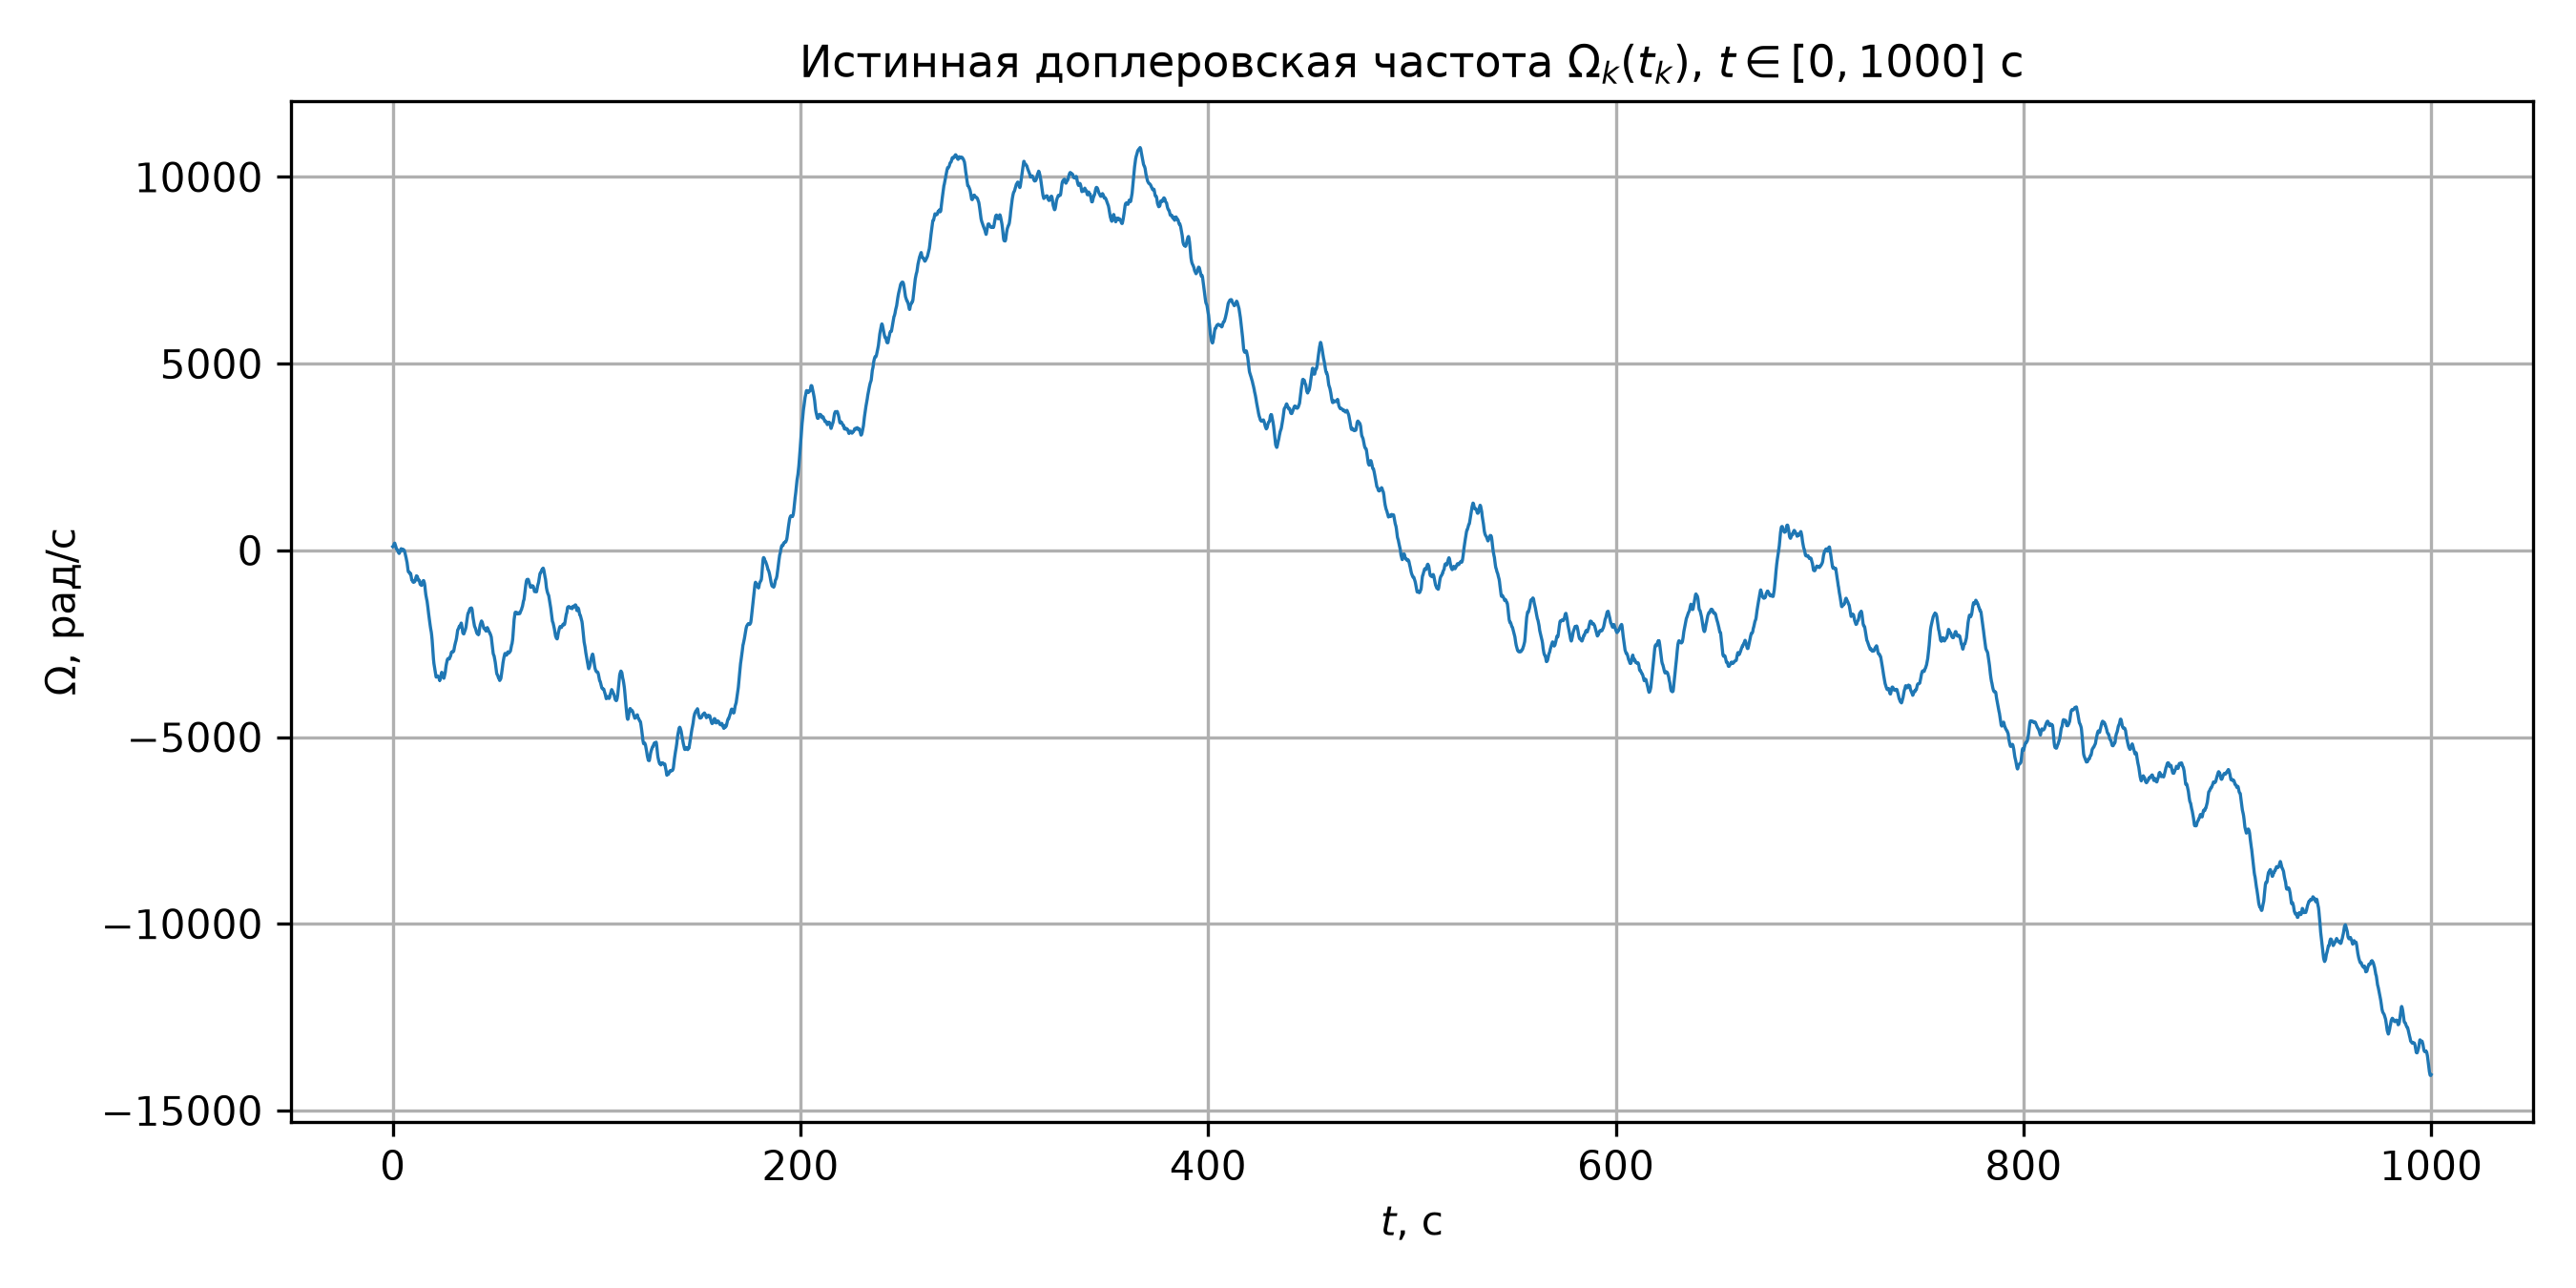
\includegraphics[width=0.85\textwidth]{1.png}
\caption{Реализация истинной доплеровской частоты $\Omega_k(t_k)$ на интервале $1000\text{ с}$}
\label{fig:omega_true}
\end{figure}

\begin{figure}[H]
\centering
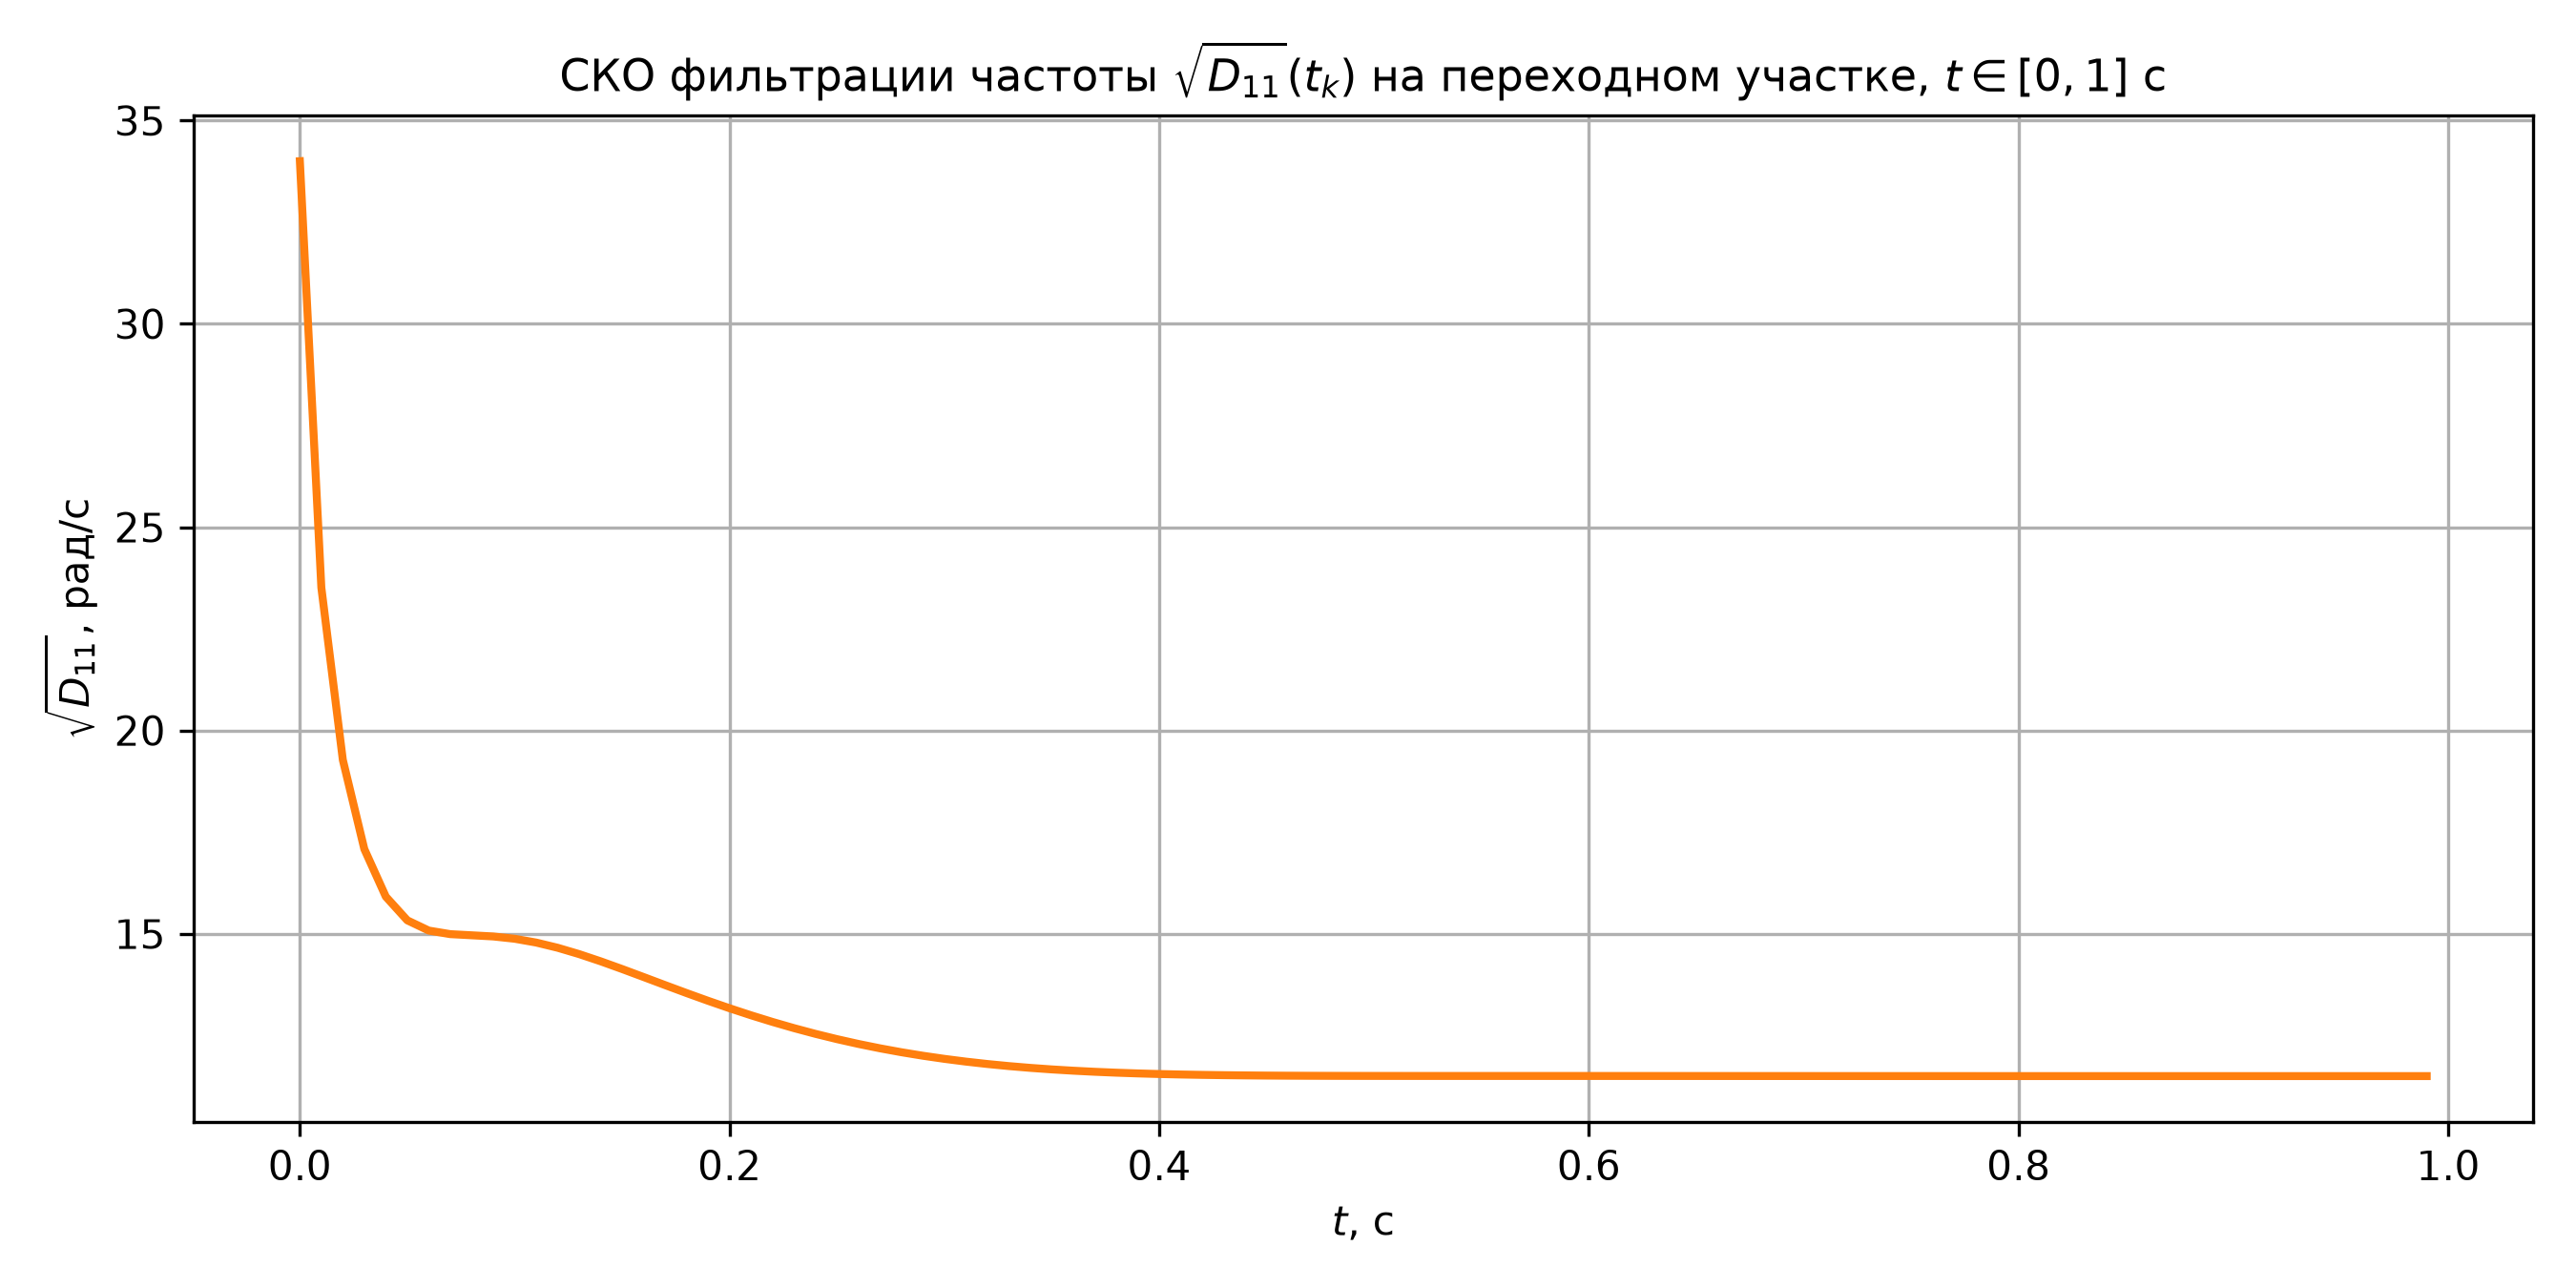
\includegraphics[width=0.85\textwidth]{2.png}
\caption{Зависимость теоретического СКО фильтрации $\sqrt{D_{11}}(t_k)$ на переходном участке}
\label{fig:sigma_transient}
\end{figure}

\begin{figure}[H]
\centering
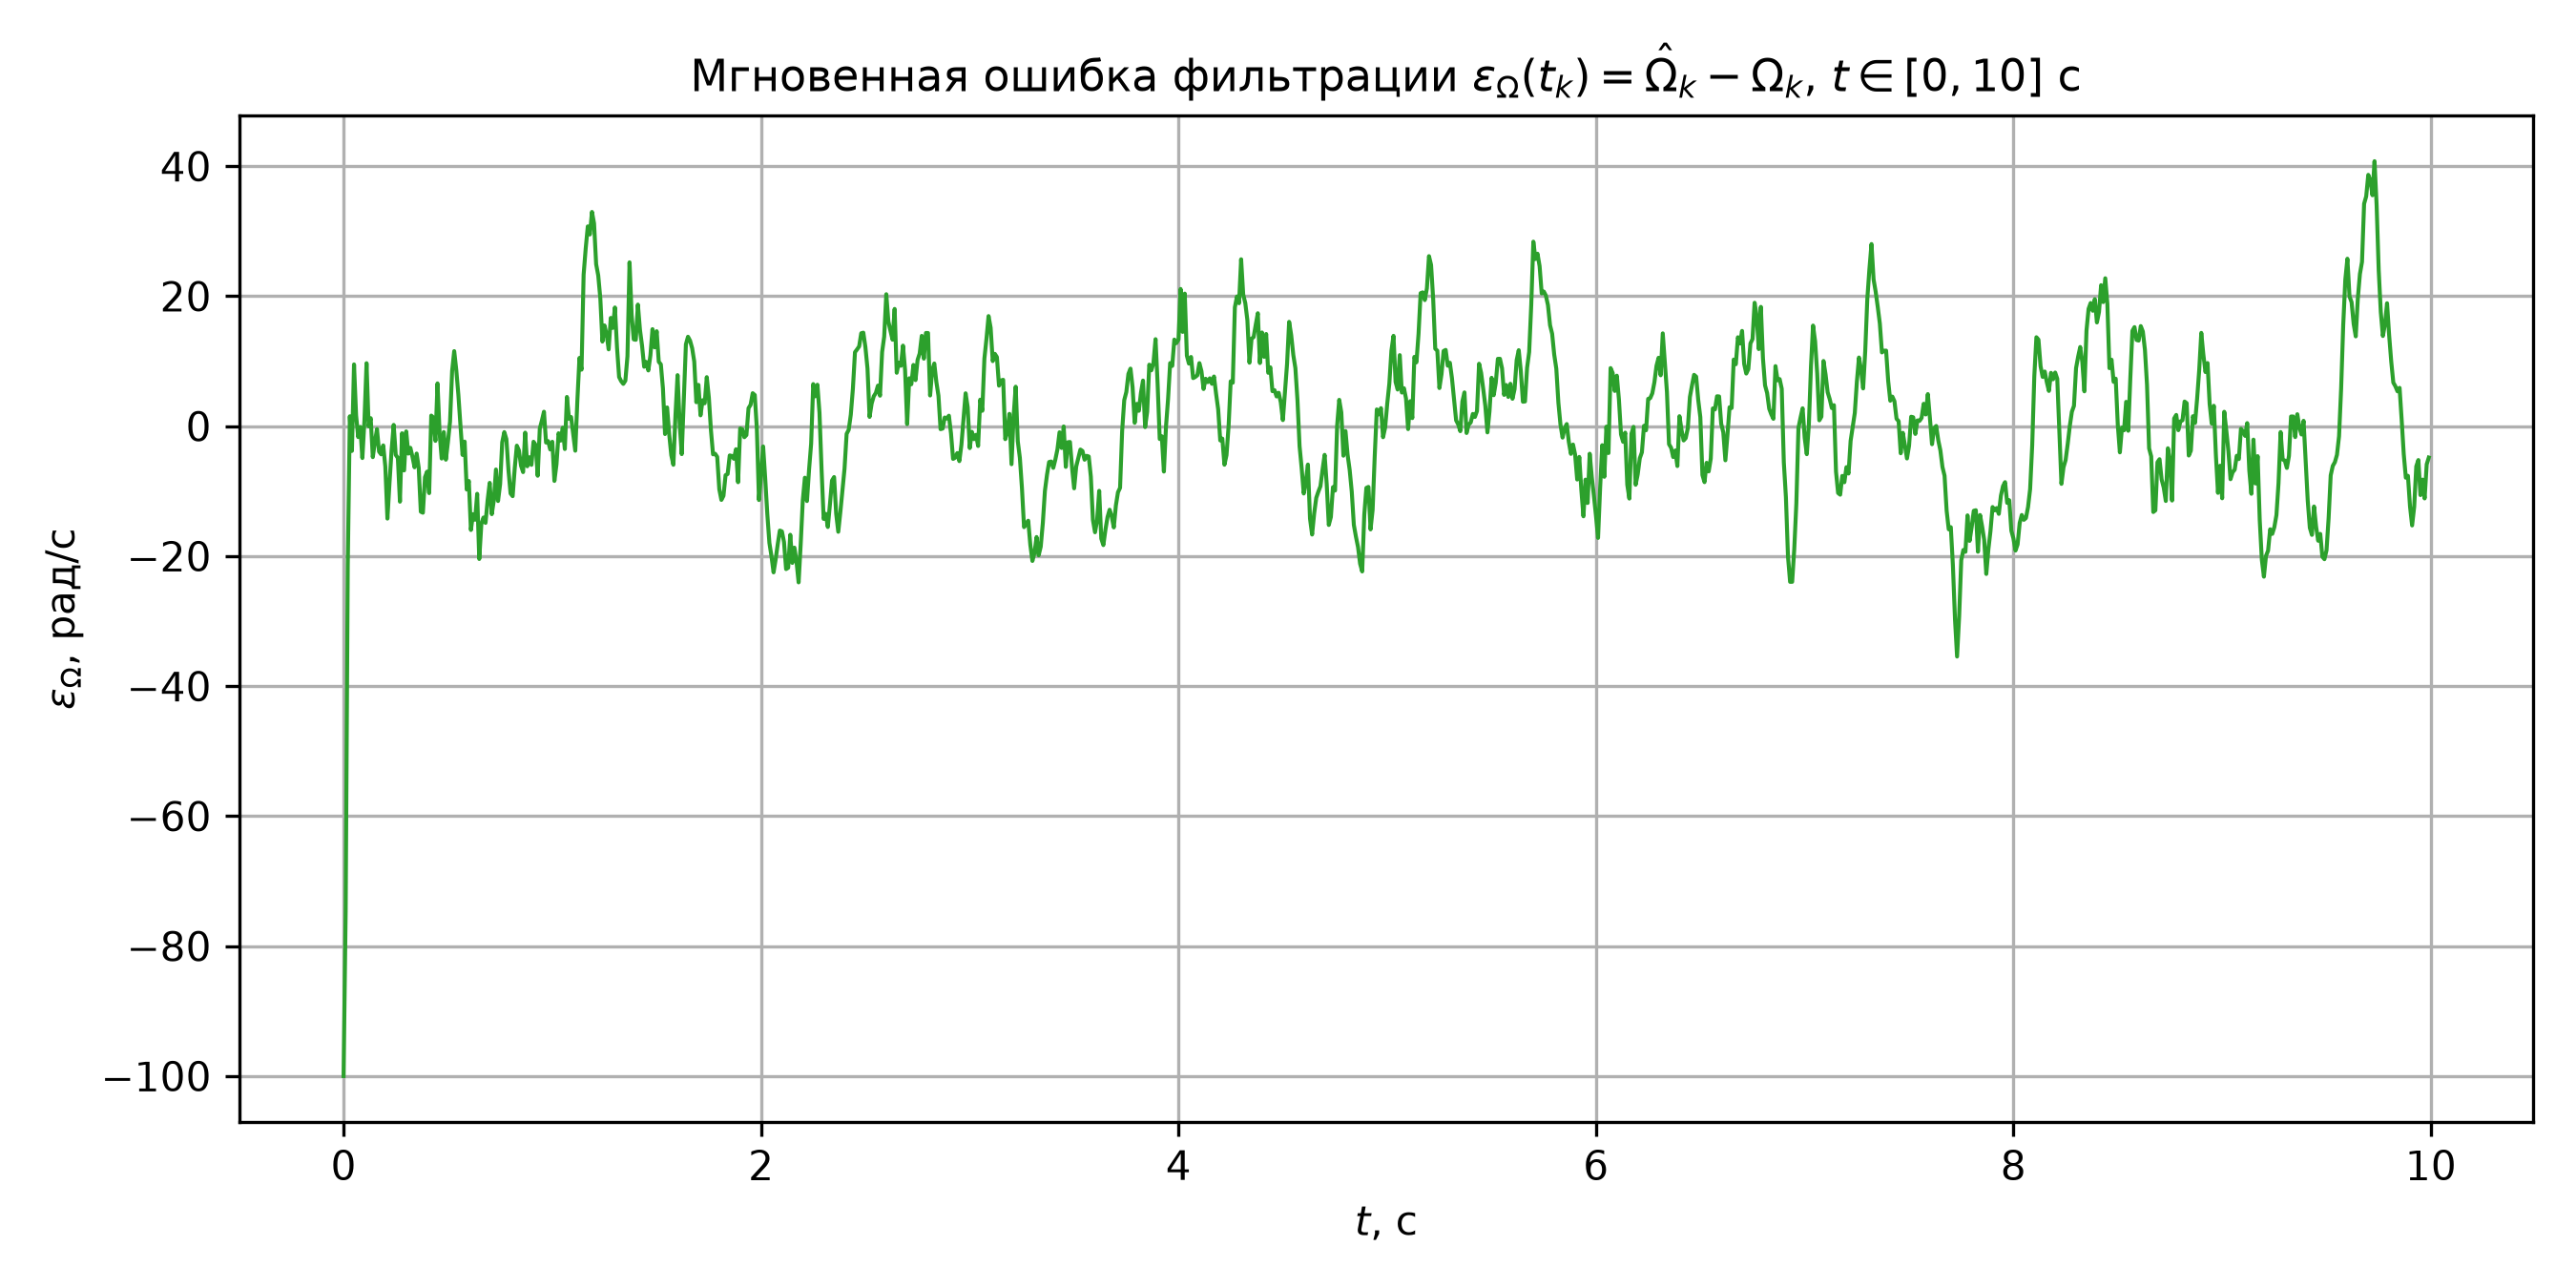
\includegraphics[width=0.85\textwidth]{3.png}
\caption{Мгновенная ошибка фильтрации доплеровской частоты $\epsilon_\Omega(t_k)$}
\label{fig:inst_error}
\end{figure}

\subsection{Сравнение теоретической и выборочной дисперсий в установившемся режиме}
Из рис.~\ref{fig:sigma_transient} и~\ref{fig:inst_error} следует, что переходный процесс завершается примерно за $0.4 \dots 0.5\text{ с}$. Для оценки стационарных характеристик отброшен начальный участок $t \in [0, 5]\text{ с}$, после чего по оставшейся выборке из $99500$ отсчетов вычислена выборочная дисперсия ошибки фильтрации. Результаты расчета и сравнения дисперсий, выведенные программой в консоль, показаны на рис.~\ref{fig:terminal_out}.

\begin{figure}[H]
\centering
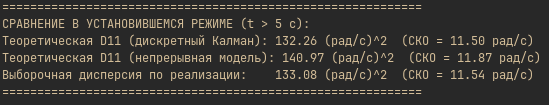
\includegraphics[width=0.85\textwidth]{6.png}
\caption{Результаты сравнения теоретической и выборочной дисперсий в установившемся режиме}
\label{fig:terminal_out}
\end{figure}

Теоретическая установившаяся дисперсия дискретного фильтра Калмана составила $D_{11,\text{теор}} = 132.26\text{ (рад/с)}^2$, что соответствует СКО $\sigma_{\Omega,\text{теор}} = 11.50\text{ рад/с}$. Аналитическая дисперсия непрерывного прототипа равна $D_{11,\text{непр}} = 140.97\text{ (рад/с)}^2$ при СКО $\sigma_{\Omega,\text{непр}} = 11.87\text{ рад/с}$. Выборочная дисперсия ошибки по смоделированной реализации составила $\hat{D}_{11,\text{эксп}} = 133.08\text{ (рад/с)}^2$, чему соответствует экспериментальное СКО $\hat{\sigma}_{\Omega,\text{эксп}} = 11.54\text{ рад/с}$.

Полученные значения практически совпадают, относительное расхождение между теоретической и выборочной дисперсиями дискретного фильтра составляет около $0.6\%$, что подтверждает корректность синтеза алгоритма. Небольшое отличие от непрерывного прототипа объясняется конечным шагом дискретизации $T = 10\text{ мс}$.
